%%%%% for latexit

\documentclass[12pt]{article}
\usepackage{booktabs}
\usepackage[dvipsnames]{xcolor} %used for font color
\usepackage{amssymb} %maths
\usepackage{amsmath} %maths
\usepackage[utf8]{inputenc} %useful to type directly diacritic characters
\nopagecolor
\color{black!0.2}

\usepackage{tikz}
\usetikzlibrary{shapes,decorations,arrows,calc,arrows.meta,fit,positioning}
\tikzset{
    -Latex,auto,node distance =1 cm and 1 cm,semithick,
    state/.style ={ellipse, draw, minimum width = 0.7 cm},
    point/.style = {circle, draw, inner sep=0.04cm,fill,node contents={}},
    bidirected/.style={Latex-Latex,dashed},
    el/.style = {inner sep=2pt, align=left, sloped}
}


%%%%% distributions
\begin{tabular}{cccc}
    %\toprule
    $H$ & $E$ & $C$ & $p(H,E,C)$\\
    \midrule
    0 & 0 & 0 & 0.027 \\
    0 & 0 & 1 & 0.102 \\
    0 & 1 & 0 & 0.504 \\
    0 & 1 & 1 & 0.076 \\
    1 & 0 & 0 & 0.003 \\
    1 & 0 & 1 & 0.068 \\
    1 & 1 & 0 & 0.216 \\
    1 & 1 & 1 & 0.004
    %\bottomrule
\end{tabular}
    
\begin{tabular}{c}
    \toprule
    $p(E=1)$\\
    \midrule
    $0.5$\\
    \bottomrule
    \end{tabular}
    
    \begin{tabular}{ccc}
    \toprule
    $E$ & $C$ & $p(H=1|E,C)$\\
    \midrule
    0 & 0 & 0.05       \\
    0 & 1 & 0.01       \\
    1 & 0 & 0.2        \\
    1 & 1 & 0.06       \\
    \bottomrule
    \end{tabular}
    
    \begin{tabular}{cc}
    \toprule
    $E$ & $p(C=1|E)$\\
    \midrule
    0 & 0.01     \\
    1 & 0.99    \\
    \bottomrule
\end{tabular}



%%%%% bayesian network

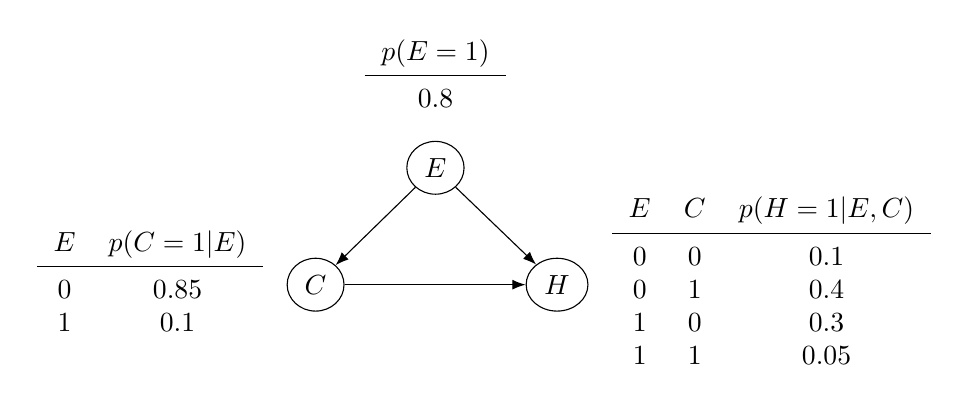
\begin{tikzpicture}
    % x node set with absolute coordinates
    \node[state] (E) at (0,0) {$E$};

    % y node set relative to x.
    % Locations can be:
    % right,left,above,below,
    % above left,below right, etc
    \node[state] (C) [below left =of E] {$C$};
    \node[state] (H) [below right =of E] {$H$};

    % Directed edge
    \path (E) edge (C);
    \path (E) edge (H);
    \path (C) edge (H);


\node [above=5pt of E]
{
\begin{tabular}{c}
%\toprule
$p(E=1)$\\
\midrule
$0.8$\\
%\bottomrule
\end{tabular}
};


\node [left=5pt of C]
{
\begin{tabular}{cc}
%\toprule
$E$ & $p(C=1|E)$\\
\midrule
0 & 0.85     \\
1 & 0.1    \\
%\bottomrule
\end{tabular}
};

\node [right=5pt of H]
{
\begin{tabular}{ccc}
%\toprule
$E$ & $C$ & $p(H=1|E,C)$\\
\midrule
0 & 0 & 0.1       \\
0 & 1 & 0.4       \\
1 & 0 & 0.3        \\
1 & 1 & 0.05       \\
%\bottomrule
\end{tabular}
};

\end{tikzpicture}


%%%%% causal graph after intervention

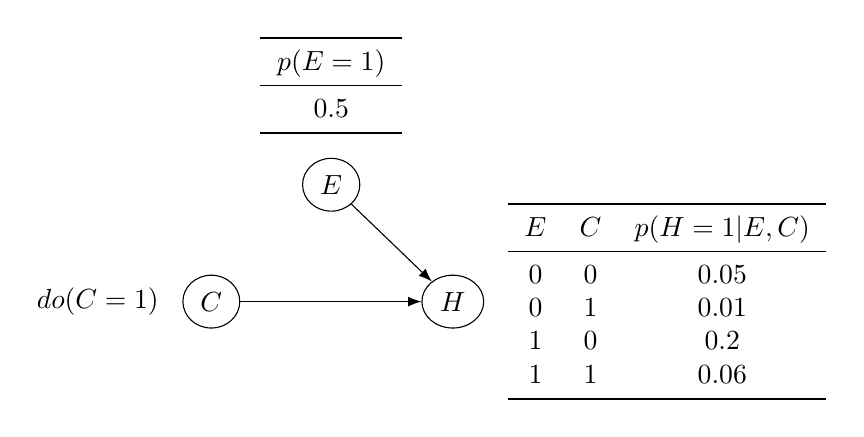
\begin{tikzpicture}
    % x node set with absolute coordinates
    \node[state] (E) at (0,0) {$E$};

    % y node set relative to x.
    % Locations can be:
    % right,left,above,below,
    % above left,below right, etc
    \node[state] (C) [below left =of E] {$C$};
    \node[state] (H) [below right =of E] {$H$};

    % Directed edge
    \path (E) edge (H);
    \path (C) edge (H);


\node [above=5pt of E]
{
\begin{tabular}{c}
\toprule
$p(E=1)$\\
\midrule
$0.5$\\
\bottomrule
\end{tabular}
};


\node [left=5pt of C]
{
$do(C=1)$
};

\node [right=5pt of H]
{
\begin{tabular}{ccc}
\toprule
$E$ & $C$ & $p(H=1|E,C)$\\
\midrule
0 & 0 & 0.05       \\
0 & 1 & 0.01       \\
1 & 0 & 0.2        \\
1 & 1 & 0.06       \\
\bottomrule
\end{tabular}
};

\end{tikzpicture}



\begin{tabular}{lllllllll}
\toprule
                        &     & \multicolumn{3}{l}{Observation}                & \multicolumn{3}{l}{Experiment}       &                          \\
                        &     & Candidates & Hired & $P(H=1|C)$ & Candidates           & Hired           & $P(H\!=\!1|do(C))$ &                   \\
\midrule
\multirow{3}{*}{$C=0$} & $E=0$ & 30         & 3     &          & 100                  & 10              &       & \multirow{3}{*}{World 0} \\
                        & $E=1$ & 720        & 216   &          & 400                  & 120             &       &                          \\
\cmidrule{3-8}
                        &     & 750        & 219   & \textbf{0.292}    & 500                  & 130             & \textbf{0.26}  &                          \\
\midrule
\multirow{3}{*}{$C=1$} & $E=0$ & 170        & 68    &          & 100                  & 40              &       & \multirow{3}{*}{World 1} \\
                        & $E=1$ & 80         & 4     &          & 400                  & 20              &       &                          \\
\cmidrule{3-8}
                        &     & 250        & 72    & \textbf{0.288}    & 500                  & 60              & \textbf{0.12}  &                         \\
\bottomrule
\end{tabular}


\begin{tabular}{llll}
$E$ & $C$ & $P(E,C)$ & $P(H=1|E,C)$ \\
0 & 0 & 0.03   & 0.1        \\
0 & 1 & 0.17   & 0.4        \\
1 & 0 & 0.72   & 0.3        \\
1 & 1 & 0.08   & 0.05      
\end{tabular}